\section{Case Study: Modularizing Language Components}
\label{sec:application}

To further illustrate the applicability of \name, we present a case
study using Object Algebras~\cite{oliveira2012extensibility} and
Extensible \textsc{Visitor}s~\cite{oliveira09modular, togersen:2004}. Encodings
of extensible designs for Object Algebras and Extensible \textsc{Visitor}s have
been presented in mainstream languages~\cite{oliveira09modular, togersen:2004, oliveira2012extensibility, oliveira2013feature, rendel14attributes}.
However, prior approaches are not entirely satisfactory
due to the limitations in existing mainstream OO languages. In \cref{sec:ob}, we show how \name makes those designs significantly simpler and
convenient to use. In particular, \name's encoding of extensible visitors gives true ASTs and supports
conflict-free Object Algebra combinators, thanks to first-class traits and disjoint polymorphism.
Based on this technique, \cref{sec:case} gives a bird-view of several orthogonal features of
a small JavaScript-like language from a textbook on Programming
Languages~\cite{poplcook}, and illustrates how various features can
be modularly developed and composed to assemble a complete language with various
operations baked in. \Cref{sec:evaluate} compares our \name's implementation
with that of the textbook using Haskell in terms of lines of code.


\subsection{Object Algebras and Extensible Visitors in \name}
\label{sec:ob}

First we give a simple introduction to Object Algebras, a design pattern that
can solve the Expression Problem~\cite{wadler1998expression} (EP) in languages like
Java. The objective of EP is to \emph{modularly} extend a datatype in two
dimensions: by adding more cases to the datatype and by adding new operations
for the datatype.
Our starting point is the following code:
\lstinputlisting[linerange=4-9]{../../examples/application.sl}% APPLY:linerange=ALGEBRA_DEF
\lstinline{ExpAlg[E]} is the generic interface of a simple arithmetic language
with two cases, \lstinline{lit} for literals and \lstinline{add} for addition.
\lstinline{ExpAlg[E]} is also called an Object Algebra interface. A concrete
Object Algebra will implement such an interface by instantiating \lstinline{E}
with a suitable type. Here we also define one operation \lstinline{IEval},
modelled by a single-field record type. A concrete Object Algebra that
implements the evaluation rules is given by a trait
\lstinline{evalAlg}.

\subparagraph{First-Class Object Algebra Values.}
The actual AST of this simple arithmetic language is given as an internal
visitor~\cite{Oliveira_2008}:
\lstinputlisting[linerange=13-13]{../../examples/application.sl}% APPLY:linerange=EXP_TYPE
Note that Object Algebras as implemented in languages like Java or Scala do not define the type
\lstinline{Exp} because this would make adding new variants very hard. Although extensible versions
of this visitor pattern do exist, they usually require complex types using advanced features of
generics~\cite{oliveira2012extensibility, togersen:2004}.
However, as we will see, this is not a problem in \name. We can build a value of \lstinline{Exp} as follows:
\lstinputlisting[linerange=17-17]{../../examples/application.sl}% APPLY:linerange=VALUE_E1


\subparagraph{Adding a New Operation.}
We add another operation \lstinline{IPrint} to the language:
\lstinputlisting[linerange=22-28]{../../examples/application.sl}% APPLY:linerange=PRINT_DEF
This is done by giving another trait \lstinline{printAlg} that implements the
additional \lstinline{print} method.


\subparagraph{Adding a New Case.}
A second dimension for extension is to add another case for negation:
\lstinputlisting[linerange=33-39]{../../examples/application.sl}% APPLY:linerange=SUB_DEF
This is achieved by extending \lstinline{evalAlg} and \lstinline{printAlg}, implementing
missing operations for negation, respectively. We define the actual AST similarly:
\lstinputlisting[linerange=44-44]{../../examples/application.sl}% APPLY:linerange=EXPEXT_TYPE
and build a value of \lstinline{-(2 + 3)} while reusing \lstinline{e1}:
\lstinputlisting[linerange=49-49]{../../examples/application.sl}% APPLY:linerange=VALUE_E2

\subparagraph{Relations between \lstinline{Exp} and \lstinline{ExpExt}}
At this stage, it is interesting to point out an interesting subtyping relation
between \lstinline{Exp} and \lstinline{ExtExp}: \lstinline{ExpExt}, though being an
\emph{extension} of \lstinline{Exp} is actually a \emph{supertype} of \lstinline{Exp}.
As Oliveira~\cite{oliveira09modular} observed, these relations are
important for legacy and performance reasons since it means that, a value of
type \lstinline{Exp} can be \emph{automatically} and \emph{safely}
coerced into a value of type \lstinline{ExpExt}, allowing some
interoperability between new functionality and legacy code.
However, to ensure type-soundness, Scala (or other common OO languages) forbids any kind of type-refinement on method
parameter types. The consequence of this is that in those languages, it is
impossible to express that \lstinline{ExtExp} is both an extension and a
supertype of \lstinline{Exp}.


% Encodings
% of extensible visitors in mainstream OO languages usually fail to
% correctly express these relations, or require sophisticated
% type system extensions~\cite{oliveira09modular}.



\subparagraph{Dynamic Object Algebra Composition Support}

When programming with Object Algebras, oftentimes it is necessary to pack
multiple operations in the same object. For example, in the simple language we
have been developing it can be useful to create an object that supports both
printing and evaluation. Oliveira and Cook~\cite{oliveira2012extensibility}
addressed this problem by proposing \emph{Object Algebra combinators} that
combine multiple algebras into one. However, as they noted, such combinators
written in Java are difficult to use in practice, and they require significant
amounts of boilerplate. Improved variants of Object Algebra combinators have
been encoded in Scala using intersection types and an encoding of the merge
construct~\cite{oliveira2013feature, rendel14attributes}. However, the
Scala encoding of the merge construct is quite complex as it relies on low-level
type-unsafe programming features such as dynamic proxies, reflection or other
meta-programming techniques. In \name, the combination of first-class
traits, dynamic inheritance and disjoint polymorphism allows type-safe, coherent
and boilerplate-free composition of Object Algebras.
\lstinputlisting[linerange=54-55]{../../examples/application.sl}% APPLY:linerange=COMBINE
That is it. None of the boilerplate in other
approaches~\cite{oliveira2012extensibility}, or type-unsafe meta-programming
techniques of other approaches~\cite{oliveira2013feature,rendel14attributes} are
needed! Two points are worth noting: (1) \lstinline{combine} relies on
\emph{dynamic inheritance}. Notice how \lstinline{combine} inherits two traits
\lstinline{f} and \lstinline{g}, for which their implementations are unknown
statically; (2) the disjointness constraint (\lstinline{B * A}) is \emph{crucial} to
ensure two Object Algebras (\lstinline{f} and \lstinline{g}) are conflict-free
when being composed.

To conclude, let us see \lstinline{combine} in action. We combine \lstinline{negEvalAlg} and \lstinline{negPrintAlg}:
\lstinputlisting[linerange=59-59]{../../examples/application.sl}% APPLY:linerange=NEW_ALG
The combined algebra \lstinline{combineAlg} is useful to avoid multiple interpretations
of the same AST when running multiple operations. For example, we can
create an object \lstinline{o} that supports both evaluation and printing in one go:
\lstinputlisting[linerange=72-73]{../../examples/application.sl}% APPLY:linerange=USE


\begin{figure}[t]
\centering
\begin{small}
\begin{tabular}{lrclr}
  Types  & $\tau$ & ::= & $ \mathsf{int}  \mid  \mathsf{bool} $ & \\
  Expressions & $e$ & ::= & $ i  \mid \,  \ottnt{e_{{\mathrm{1}}}}  \ottsym{+}  \ottnt{e_{{\mathrm{2}}}} \mid \,  \ottnt{e_{{\mathrm{1}}}}  \ottsym{-}  \ottnt{e_{{\mathrm{2}}}} \mid \,  \ottnt{e_{{\mathrm{1}}}}  \times  \ottnt{e_{{\mathrm{2}}}} \mid \,  \ottnt{e_{{\mathrm{1}}}}  \div  \ottnt{e_{{\mathrm{2}}}} $ & $\mathit{natF}$ \\
              && $\mid$ & $ \mathbb{B}  \mid \ottkw{if} \, \ottnt{e_{{\mathrm{1}}}} \, \ottkw{then} \, \ottnt{e_{{\mathrm{2}}}} \, \ottkw{else} \, \ottnt{e_{{\mathrm{3}}}} $ & $\mathit{boolF}$\\
              && $\mid$ & $ \,  \ottnt{e_{{\mathrm{1}}}}  \ottsym{==}  \ottnt{e_{{\mathrm{2}}}} \mid \,  \ottnt{e_{{\mathrm{1}}}}  \ottsym{<}  \ottnt{e_{{\mathrm{2}}}} $ & $\mathit{compF}$ \\
              && $\mid$ & $ \,  \ottnt{e_{{\mathrm{1}}}}  \,\&\&\,  \ottnt{e_{{\mathrm{2}}}} \mid \,  \ottnt{e_{{\mathrm{1}}}}  \,||\,  \ottnt{e_{{\mathrm{2}}}} $ & $\mathit{logicF}$ \\
              && $\mid$ & $\ottmv{x} \mid \ottkw{var} \, \ottmv{x}  \ottsym{=}  \ottnt{e_{{\mathrm{1}}}}  \ottsym{;}  \ottnt{e_{{\mathrm{2}}}}$  &  $\mathit{varF}$ \\
              && $\mid$ & $\,  \ottnt{e_{{\mathrm{1}}}} \, \ottnt{e_{{\mathrm{2}}}}$ & $\mathit{funcF}$ \\
  Programs & $pgm$ & ::= & $decl_{{\mathrm{1}}} \dots decl_{\ottmv{n}} \, \ottnt{e}$ &  $\mathit{funcF}$ \\
  Functions & $decl$ & ::= & $\ottkw{function} \, \ottmv{f}  \ottsym{(}  \ottmv{x}  \ottsym{:}  \tau  \ottsym{)}  \ottsym{\{}  \ottnt{e}  \ottsym{\}}$ &  $\mathit{funcF}$ \\
  Values & $v$ & ::= & $ i  \mid  \mathbb{B} $ &
\end{tabular}

\end{small}
\caption{Mini-JS expressions, values, and types}
\label{fig:mini-js}
\end{figure}

\subsection{Case Study Overview}
\label{sec:case}

Now we are ready to see how the same technique scales to modularize different
language features. A \emph{feature} is an increment in program
functionality~\cite{zave1999faq,lopez2005evaluating}. \Cref{fig:mini-js}
presents the syntax of the expressions, values and types provided by the
features; each line is annotated with the corresponding feature name. Starting from a
simple arithmetic language, we gradually introduce new features and combine them
with some of the existing features to form various languages. Below we briefly
explain what constitutes each feature:
\begin{itemize}
\item $\mathit{natF}$ and $\mathit{boolF}$ contain, among others, literals, additions and conditional expressions.
\item $\mathit{compF}$ and $\mathit{logicF}$ introduce comparisons between numbers and logical connectives.
\item $\mathit{varF}$ introduces local variables and variable declarations.
\item $\mathit{funcF}$ introduces top-level functions and function calls.
\end{itemize}
Besides, each feature is packed with 3 operations: evaluator, pretty
printer and type checker.

Having the feature set, we can synthesize different languages by selecting one
or more operations, and one or more data variants, as shown in \cref{fig:langs}.
For example \lstinline{arith} is a simple language of arithmetic expressions,
assembled from $\mathit{natF}$, $\mathit{boolF}$ and $\mathit{compF}$. On top of
that, we also define an evaluator, a pretty printer and a type checker. Note
that for some languages (e.g., \lstinline{simplenat}), since they have only one
kind of value, we only define an evaluator and a pretty printer. We thus obtain
12 languages and 30 operations in total. The complete language
\lstinline{mini-JS} contains all the features and supports all the operations. % Besides, we also define
% a new algebra with the combined behavior of all the operations.
The reader can refer to our supplementary material for the source code of the case study.


\begin{figure}[t]
  \centering
  \begin{small}
\begin{tabular}{|l||c|c|c||c|c|c|c|c|c|}
\hline
\multirow{2}{*}{Language} & \multicolumn{3}{c||}{Operations} & \multicolumn{6}{c|}{Data variants}           \\ \cline{2-10}
                      & eval     & print     & check    & $\mathit{natF}$ & $\mathit{boolF}$ & $\mathit{compF}$ & $\mathit{logicF}$ & $\mathit{varF}$ & $\mathit{funcF}$ \\ \hline \hline
\lstinline$simplenat$             &   \cmark       & \cmark          &          &  \cmark    &       &       &        &      &       \\ \hline
\lstinline$simplebool$          &  \cmark        &  \cmark         &          &      &  \cmark     &       &        &      &       \\ \hline
\lstinline$natbool$       &  \cmark        & \cmark          & \cmark         & \cmark     & \cmark      &       &        &      &       \\ \hline
\lstinline$varbool$       &  \cmark        &  \cmark         &          &      & \cmark      &       &        & \cmark     &       \\ \hline
\lstinline$varnat$      &   \cmark       &  \cmark         &   &  \cmark    &     &       &        & \cmark      &       \\ \hline
\lstinline$simplelogic$  &  \cmark        &  \cmark         &          &      &   \cmark    &       &    \cmark    &      &       \\ \hline
\lstinline$varlogic$   &    \cmark      &   \cmark        &          &      &  \cmark     &       &  \cmark  &  \cmark    &       \\ \hline
\lstinline$arith$     &  \cmark  &  \cmark &  \cmark &  \cmark    &  \cmark     &  \cmark     &        &      &       \\ \hline
\lstinline$arithlogic$ &  \cmark   &  \cmark &  \cmark  & \cmark     &  \cmark     & \cmark      & \cmark       &      &       \\ \hline
\lstinline$vararith$        &  \cmark   &  \cmark  &  \cmark  & \cmark     &  \cmark     &  \cmark     &        & \cmark     &       \\ \hline
\lstinline$vararithlogic$  &  \cmark &  \cmark  &  \cmark  & \cmark & \cmark & \cmark &  \cmark & \cmark &       \\ \hline
\lstinline$mini-JS$  &  \cmark &  \cmark  &  \cmark  & \cmark & \cmark & \cmark &  \cmark & \cmark & \cmark      \\ \hline
\end{tabular}

  \end{small}
\caption{Overview of the languages assembled}
\label{fig:langs}
\end{figure}




% \cref{fig:dependency} gives an overview of the reusable components of the
% implementation, and the subtyping/inheritance relations of the languages we can
% assemble. The interactions between languages and features are revealed by the
% arrows. Below we briefly explain what features/operations each language supports:
% \begin{itemize}
% \item \lstinline{ArithL} is a simple language of arithmetic expressions,
%   directly inherited from the feature $\mathit{Arith}$. We define an evaluator
%   and a pretty printer.
% \item \lstinline{BoolArithL} extends \lstinline{ArithL} with the feature
%   $\mathit{Bool}$. Apart from the evaluator and pretty printer, we define
%   another operation: type checker. Thus \lstinline{BoolArithL} is illustrative
%   of solving the Expression Problem.
% \item \lstinline{VarArithL} extends \lstinline{BoolArithL} with the feature
%   $\mathit{Var}$. We define an evaluator, a pretty printer, and a type checker.
% \item \lstinline{Mini-JS} is the complete language that inherits all the
%   features and operations.
% \end{itemize}

% From \cref{fig:langs} we can also see the subtyping/inheritance relations
% between each language. For example, since the feature set of \lstinline{arith}
% is a super set of that of \lstinline{natbool}, we can say \lstinline{arith} extends
% \lstinline{natbool}, and the former is a supertype of the latter. Indeed,
% operations defined for \lstinline{arith} can safely apply to expressions of \lstinline{natbool}.


% For example, the leftward arrow between
% \lstinline{BoolArithL} and \lstinline{ArithL} says that \lstinline{BoolArithL}
% extends \lstinline{ArithL}, while the rightward dashed arrow between them says
% that \lstinline{ArithL} is a subtype of \lstinline{BoolArithL}. We thus obtain 4
% languages and 11 operations in total.

% \begin{figure}[t]
%   \centering
%   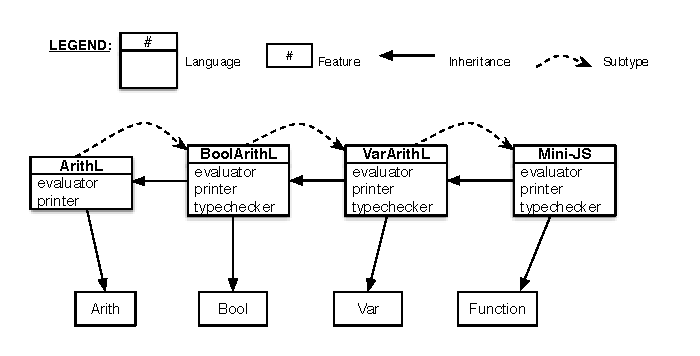
\includegraphics{dependency.eps}
%   \caption{Overview of the language components.}
%   \label{fig:dependency}
% \end{figure}

\subsection{Evaluation}
\label{sec:evaluate}

To evaluate \name's implementation of the case study,
\Cref{fig:sloc} compares the number of source lines of code
(SLOC, lines of code without counting empty lines and comments) for
\name's \emph{modular} implementation with the vanilla
\emph{non-modular} AST-based implementations in Haskell. The Haskell
implementations are just straightforward AST interpreters, which duplicate code across the multiple language
components.

Since \name is a new language, we
had to write various code that is provided in Haskell by the standard library,
so they are not counted for fairness of comparison. In the left part, for each
feature, we count the lines of the algebra interface (number beside the feature
name), and the algebras for the operations. In the right part, for each
language, we count the lines of ASTs, and those to combine previously
defined operations. For example, here is the code that is needed to make the
\lstinline{arith} language.
\lstinputlisting[linerange=537-544]{../../examples/case_study.sl}% APPLY:linerange=ARITH
We only need 8 lines in total: 2 lines for the AST, and 6 lines to combine the operations.

Therefore, the total SLOC of \name's implementation is the sum of all the
lines in the feature and language parts (237 SLOC of all features plus 94 SLOC
of ASTs and operations). Although \name is considerably more verbose than a
functional language like Haskell, \name's modular implementation for 12 languages and 30
operations in total reduces approximately 60\% in terms of SLOC. The reason is
that, the more frequently a feature is reused by other languages directly or
indirectly, the more reduction we see in the total SLOC. For example,
$\mathit{natF}$ is used across many languages. Even though \lstinline{simplenat}
itself \emph{alone} has more SLOC ($40 = 7+23+7+3$) than that of Haskell (which
has 33), we still get a huge gain when implementing other languages.

Finally, we acknowledge the limitation of our case study in that SLOC is just
one metric and we have not measured any other metrics. Nevertheless we believe
that the case study is already non-trivial in that we need to solve EP. Note
that Scala traits alone are not sufficient on their own to solve EP. While there
are solutions to EP in both Haskell and Scala, they
introduce significant complexity, as explained in \cref{sec:ob}.



\begin{figure}[t]
  \centering
  \begin{small}
  \begin{tabular}{|r|ccc||l|ccc|}
    \hline
     Feature & \textbf{eval} & \textbf{print} & \textbf{check} & Lang name & \name & \textbf{Haskell} & \textbf{\% Reduced}  \\
    \hline
    $\mathit{natF}$(7) & 23 & 7 & 39 & \lstinline$simplenat$ & 3 & 33 & 91\%  \\
    $\mathit{boolF}$(4) & 9 & 4 & 17 & \lstinline$simplebool$ & 3 & 16 & 81\% \\
    $\mathit{compF}$(4) & 12 & 4 & 20 & \lstinline$natbool$ & 5 & 74 & 93\% \\
    $\mathit{logicF}$(4) & 12 & 4 & 20 & \lstinline$varbool$ & 4 & 24 & 83\% \\
    $\mathit{varF}$(4) & 7 & 4 & 7 & \lstinline$varnat$ & 4 & 41 & 90\% \\
    $\mathit{funcF}$(3) & 10 & 3 & 9 & \lstinline$simplelogic$ & 4 & 28 & 86\% \\
     & & & & \lstinline$varlogic$ & 6 & 36 & 83\% \\
     & & & & \lstinline$arith$ & 8 & 94 & 91\% \\
     & & & & \lstinline$arithlogic$ & 8 & 114 & 93\% \\
     & & & & \lstinline$vararith$ & 8 & 107 & 93\% \\
     & & & & \lstinline$vararithlogic$ & 8 & 127 & 94\% \\
     & & & & \lstinline$mini-JS$ & 33 & 149 & 78\% \\
    \hline
    \bf{Total} & & & 237 & & 331 & 843 & 61\% \\
    \hline
  \end{tabular}
  \end{small}
  \caption{SLOC statistics: \name implementation vs vanilla AST implementation.}
  \label{fig:sloc}
\end{figure}




\begin{comment}
\subsection{Putting all together}

% With all the components ready, we can assemble them at will to cook a language
% with whatever features we want. For example, we hope by now the reader can share
% our feeling that this is indeed a simple and modular way to cook a language
% incrementally.

To demonstrate the usage of the final language \lstinline{MiniJS}, here is a function that
makes sure ``well-typed programs cannot go wrong'':
\lstinputlisting[linerange=-]{}% APPLY:linerange=SUPER_DEF
It type checks the program before passing it to the evaluator and pretty
printer.

% we first create a program that
% uses all the features the language supports now.
% \lstinputlisting[linerange=-]{}% APPLY:linerange=FINAL_TEST
% The concrete syntax of the program is shown in the comment above. We assume a
% pre-defined function environment (\lstinline{fenv}) containing the definition of
% the \lstinline{add1} function.

% Finally we apply it to the program we have just created:
% \lstinputlisting[linerange=735-736]{../../examples/case_study.sl}% APPLY:linerange=TEST_TEST
% Everything works as expected!
\end{comment}

\begin{comment}
\subsection{Parameterizing Expressions by the Evaluation Order}

We now turn to the second case study. In this case study, we embed a
higher-order domain-specific language inside \name. Our object language in this
case study is typed lambda calculus with conditional and constants. This time,
the embedding not only demonstrates the extensibility, as is shown in the first
case study, but also object types, expressed in the meta-language (\name) and
manifestly ensuring well-scoped and well-typed expressions in the object
language. What is more, the evaluator over the object expressions is type
preserving by construction. The embedding of typed languages is directly
inspired by Kiselyov's lecture notes~\cite{kiselyov2012typed} on the
"tagless-final" approach to embedding languages.

\paragraph{Well-typed object expressions} One important issue with such
embedding is how to deal with binders in the object language. In general there
are two options, one can either use deBrujin indices~\cite{}, or higher-order
abstract syntax (HOAS)~\cite{}. Each option has its cons and pros, but for this
particular case study, we find HOAS convenient. HOAS represents object language
abstractions as \name abstractions and object variables as \name variables. By
utilizing the infrastructure of the meta-language, we are free of issues such as
variable capture. Here is the interface of the object language.
\lstinputlisting[linerange=-]{}% APPLY:linerange=TYPED_LAMBDA
Embedded object expressions of type \lstinline{A} are represented as \name
values of the type \lstinline{Expr[A]}. The \lstinline{bot} constructor, which
represents non-terminating computation, is there for the purpose of illustrating
different evaluation strategies.

A careful reader may notice that the \lstinline{ExprAlg} interface has no
abstractions. This is intentional! Evaluators with different evaluation
strategies only differ in the interpretation for abstractions, as will be shown
later on. For this reason, \lstinline{lam} is moved to a separate interface of
its own.
\lstinputlisting[linerange=-]{}% APPLY:linerange=ABSTRACTION


\paragraph{Well-typed evaluator}
The benefit of typeful embedding shows up when defining the evaluator.
\lstinputlisting[linerange=-]{}% APPLY:linerange=TYPED_EVAL
Unlike the evaluator in the first case study, there is no need for a separate
\lstinline{Value} datatype for values, as they are directly modeled by \name
values. Note that the resulting evaluator is \emph{type preserving} by
construction.

\paragraph{Call-by-name, call-by-value}
Our evaluator defined in the first case study inherits the evaluation strategy
from the meta-language. We now show call-by-name and call-by-value evaluators.
The two evaluators are quite alike, sharing most of the code. As said before,
the only difference is the interpretation for \lstinline{lam}.
\lstinputlisting[linerange=-]{}% APPLY:linerange=CBN_CBV
The call-by-name \lstinline{lam}, when applied, will receive an unevaluated
argument expression, use it as it is. The call-by-value \lstinline{lam}, as in
the call-by-name evaluator, receives an unevaluated argument expression,
evaluates it before passing its result to the abstraction body \lstinline{f}.

Now to make an evaluator parameterized over the evaluation order, we just take a
trait \lstinline{o} with unknown implementation, compose it with other language
features.
\lstinputlisting[linerange=-]{}% APPLY:linerange=MAKE_EVAL
Here is the call-by-name evaluator at work:
\lstinputlisting[linerange=-]{}% APPLY:linerange=CBN_TEST
On the other hand, \lstinline{(evaluator evalBindCBV ex)()} would result in a
infinite loop. The complete code with several examples can be found in the
supplementary materials.

\jeremy{I am afraid we don't seem to have many advantages over OCaml's version,
  because we don't really have higher-kinded types, we cannot make a AST type
  for this example, though \lstinline{makeEvaluator} seems to be one advantage }

\end{comment}

%%% Local Variables:
%%% mode: latex
%%% TeX-master: "../paper"
%%% org-ref-default-bibliography: ../paper.bib
%%% End:
